% Options for packages loaded elsewhere
\PassOptionsToPackage{unicode}{hyperref}
\PassOptionsToPackage{hyphens}{url}
%
\documentclass[
  man,floatsintext]{apa7}
\usepackage{amsmath,amssymb}
\usepackage{iftex}
\ifPDFTeX
  \usepackage[T1]{fontenc}
  \usepackage[utf8]{inputenc}
  \usepackage{textcomp} % provide euro and other symbols
\else % if luatex or xetex
  \usepackage{unicode-math} % this also loads fontspec
  \defaultfontfeatures{Scale=MatchLowercase}
  \defaultfontfeatures[\rmfamily]{Ligatures=TeX,Scale=1}
\fi
\usepackage{lmodern}
\ifPDFTeX\else
  % xetex/luatex font selection
\fi
% Use upquote if available, for straight quotes in verbatim environments
\IfFileExists{upquote.sty}{\usepackage{upquote}}{}
\IfFileExists{microtype.sty}{% use microtype if available
  \usepackage[]{microtype}
  \UseMicrotypeSet[protrusion]{basicmath} % disable protrusion for tt fonts
}{}
\makeatletter
\@ifundefined{KOMAClassName}{% if non-KOMA class
  \IfFileExists{parskip.sty}{%
    \usepackage{parskip}
  }{% else
    \setlength{\parindent}{0pt}
    \setlength{\parskip}{6pt plus 2pt minus 1pt}}
}{% if KOMA class
  \KOMAoptions{parskip=half}}
\makeatother
\usepackage{xcolor}
\usepackage{graphicx}
\makeatletter
\def\maxwidth{\ifdim\Gin@nat@width>\linewidth\linewidth\else\Gin@nat@width\fi}
\def\maxheight{\ifdim\Gin@nat@height>\textheight\textheight\else\Gin@nat@height\fi}
\makeatother
% Scale images if necessary, so that they will not overflow the page
% margins by default, and it is still possible to overwrite the defaults
% using explicit options in \includegraphics[width, height, ...]{}
\setkeys{Gin}{width=\maxwidth,height=\maxheight,keepaspectratio}
% Set default figure placement to htbp
\makeatletter
\def\fps@figure{htbp}
\makeatother
\setlength{\emergencystretch}{3em} % prevent overfull lines
\providecommand{\tightlist}{%
  \setlength{\itemsep}{0pt}\setlength{\parskip}{0pt}}
\setcounter{secnumdepth}{-\maxdimen} % remove section numbering
% Make \paragraph and \subparagraph free-standing
\ifx\paragraph\undefined\else
  \let\oldparagraph\paragraph
  \renewcommand{\paragraph}[1]{\oldparagraph{#1}\mbox{}}
\fi
\ifx\subparagraph\undefined\else
  \let\oldsubparagraph\subparagraph
  \renewcommand{\subparagraph}[1]{\oldsubparagraph{#1}\mbox{}}
\fi
\newlength{\cslhangindent}
\setlength{\cslhangindent}{1.5em}
\newlength{\csllabelwidth}
\setlength{\csllabelwidth}{3em}
\newlength{\cslentryspacingunit} % times entry-spacing
\setlength{\cslentryspacingunit}{\parskip}
\newenvironment{CSLReferences}[2] % #1 hanging-ident, #2 entry spacing
 {% don't indent paragraphs
  \setlength{\parindent}{0pt}
  % turn on hanging indent if param 1 is 1
  \ifodd #1
  \let\oldpar\par
  \def\par{\hangindent=\cslhangindent\oldpar}
  \fi
  % set entry spacing
  \setlength{\parskip}{#2\cslentryspacingunit}
 }%
 {}
\usepackage{calc}
\newcommand{\CSLBlock}[1]{#1\hfill\break}
\newcommand{\CSLLeftMargin}[1]{\parbox[t]{\csllabelwidth}{#1}}
\newcommand{\CSLRightInline}[1]{\parbox[t]{\linewidth - \csllabelwidth}{#1}\break}
\newcommand{\CSLIndent}[1]{\hspace{\cslhangindent}#1}
\ifLuaTeX
\usepackage[bidi=basic]{babel}
\else
\usepackage[bidi=default]{babel}
\fi
\babelprovide[main,import]{english}
% get rid of language-specific shorthands (see #6817):
\let\LanguageShortHands\languageshorthands
\def\languageshorthands#1{}
% Manuscript styling
\usepackage{upgreek}
\captionsetup{font=singlespacing,justification=justified}

% Table formatting
\usepackage{longtable}
\usepackage{lscape}
% \usepackage[counterclockwise]{rotating}   % Landscape page setup for large tables
\usepackage{multirow}		% Table styling
\usepackage{tabularx}		% Control Column width
\usepackage[flushleft]{threeparttable}	% Allows for three part tables with a specified notes section
\usepackage{threeparttablex}            % Lets threeparttable work with longtable

% Create new environments so endfloat can handle them
% \newenvironment{ltable}
%   {\begin{landscape}\centering\begin{threeparttable}}
%   {\end{threeparttable}\end{landscape}}
\newenvironment{lltable}{\begin{landscape}\centering\begin{ThreePartTable}}{\end{ThreePartTable}\end{landscape}}

% Enables adjusting longtable caption width to table width
% Solution found at http://golatex.de/longtable-mit-caption-so-breit-wie-die-tabelle-t15767.html
\makeatletter
\newcommand\LastLTentrywidth{1em}
\newlength\longtablewidth
\setlength{\longtablewidth}{1in}
\newcommand{\getlongtablewidth}{\begingroup \ifcsname LT@\roman{LT@tables}\endcsname \global\longtablewidth=0pt \renewcommand{\LT@entry}[2]{\global\advance\longtablewidth by ##2\relax\gdef\LastLTentrywidth{##2}}\@nameuse{LT@\roman{LT@tables}} \fi \endgroup}

% \setlength{\parindent}{0.5in}
% \setlength{\parskip}{0pt plus 0pt minus 0pt}

% Overwrite redefinition of paragraph and subparagraph by the default LaTeX template
% See https://github.com/crsh/papaja/issues/292
\makeatletter
\renewcommand{\paragraph}{\@startsection{paragraph}{4}{\parindent}%
  {0\baselineskip \@plus 0.2ex \@minus 0.2ex}%
  {-1em}%
  {\normalfont\normalsize\bfseries\itshape\typesectitle}}

\renewcommand{\subparagraph}[1]{\@startsection{subparagraph}{5}{1em}%
  {0\baselineskip \@plus 0.2ex \@minus 0.2ex}%
  {-\z@\relax}%
  {\normalfont\normalsize\itshape\hspace{\parindent}{#1}\textit{\addperi}}{\relax}}
\makeatother

% \usepackage{etoolbox}
\makeatletter
\patchcmd{\HyOrg@maketitle}
  {\section{\normalfont\normalsize\abstractname}}
  {\section*{\normalfont\normalsize\abstractname}}
  {}{\typeout{Failed to patch abstract.}}
\patchcmd{\HyOrg@maketitle}
  {\section{\protect\normalfont{\@title}}}
  {\section*{\protect\normalfont{\@title}}}
  {}{\typeout{Failed to patch title.}}
\makeatother

\usepackage{xpatch}
\makeatletter
\xapptocmd\appendix
  {\xapptocmd\section
    {\addcontentsline{toc}{section}{\appendixname\ifoneappendix\else~\theappendix\fi\\: #1}}
    {}{\InnerPatchFailed}%
  }
{}{\PatchFailed}
\keywords{psychopathy, borderline personality disorder, alexithymia, incarcerated populations, women, psychopathology\newline\indent Word count: X}
\usepackage{lineno}

\linenumbers
\usepackage{csquotes}
\makeatletter
\renewcommand{\paragraph}{\@startsection{paragraph}{4}{\parindent}%
  {0\baselineskip \@plus 0.2ex \@minus 0.2ex}%
  {-1em}%
  {\normalfont\normalsize\bfseries\typesectitle}}

\renewcommand{\subparagraph}[1]{\@startsection{subparagraph}{5}{1em}%
  {0\baselineskip \@plus 0.2ex \@minus 0.2ex}%
  {-\z@\relax}%
  {\normalfont\normalsize\bfseries\itshape\hspace{\parindent}{#1}\textit{\addperi}}{\relax}}
\makeatother

\ifLuaTeX
  \usepackage{selnolig}  % disable illegal ligatures
\fi
\IfFileExists{bookmark.sty}{\usepackage{bookmark}}{\usepackage{hyperref}}
\IfFileExists{xurl.sty}{\usepackage{xurl}}{} % add URL line breaks if available
\urlstyle{same}
\hypersetup{
  pdftitle={Psychopathy, borderline personality disorder, and emotional processing in incarcerated women},
  pdfauthor={Annalise S Halverson1 \& Natalie Dowling1,2},
  pdflang={en-EN},
  pdfkeywords={psychopathy, borderline personality disorder, alexithymia, incarcerated populations, women, psychopathology},
  hidelinks,
  pdfcreator={LaTeX via pandoc}}

\title{Psychopathy, borderline personality disorder, and emotional processing in incarcerated women}
\author{Annalise S Halverson\textsuperscript{1} \& Natalie Dowling\textsuperscript{1,2}}
\date{}


\shorttitle{psychopathy and psychopathology correlates in women}

\authornote{

Add complete departmental affiliations for each author here. Each new line herein must be indented, like this line.

Enter author note here.

The authors made the following contributions. Annalise S Halverson: Conceptualization, Writing - Original Draft Preparation, Writing - Review \& Editing; Natalie Dowling: Writing - Review \& Editing, Supervision.

Correspondence concerning this article should be addressed to Annalise S Halverson, 5848 S University Ave, Chicago, IL, 60637. E-mail: \href{mailto:asdh@uchicago.edu}{\nolinkurl{asdh@uchicago.edu}}

}

\affiliation{\vspace{0.5cm}\textsuperscript{1} University of Chicago\\\textsuperscript{2} Department of Psychology}

\abstract{%
One or two sentences providing a \textbf{basic introduction} to the field, comprehensible to a scientist in any discipline.
Two to three sentences of \textbf{more detailed background}, comprehensible to scientists in related disciplines.
One sentence clearly stating the \textbf{general problem} being addressed by this particular study.
One sentence summarizing the main result (with the words ``\textbf{here we show}'' or their equivalent).
Two or three sentences explaining what the \textbf{main result} reveals in direct comparison to what was thought to be the case previously, or how the main result adds to previous knowledge.
One or two sentences to put the results into a more \textbf{general context}.
Two or three sentences to provide a \textbf{broader perspective}, readily comprehensible to a scientist in any discipline.
}



\begin{document}
\maketitle

\hypertarget{introduction}{%
\section{Introduction}\label{introduction}}

Psychopathy as a construct has undergone detailed iterations to annotate its numerous idiosyncrasies. Around 1.2\% of American men and 0.5\% of American women are believed to possess clinically significant levels of psychopathic traits (Barbara Burton \& Fabian M. Saleh, 2020). While persistent antisocial conduct is commonly present, psychopathy is also uniquely characterized by absences -- notably a deficiency in emotional reaction and a lack of empathy or remorse (De Brito et al., 2021; Sellbom \& Drislane, 2021). It spans race, gender, socioeconomic status, and culture, and further possesses a kaleidoscope of consequences -- from disturbed well-being to increased involvement in the criminal justice system. While it is believed to be present in around 1\% of the general population, an estimated 15-25\% of those incarcerated are likely to fall somewhere on the psychopathy spectrum (Barbara Burton \& Fabian M. Saleh, 2020).

A discrimination in subtypes of psychopathy was pioneered by Karpman (1941), who proposed the existence of two groups: primary and secondary. Primary psychopaths are exceedingly low in anxiety and predisposed to be antisocial, whereas secondary psychopaths become callous and high in anxiety as a response to various vulnerabilities in the environment (Sellbom \& Drislane, 2021). The most widely investigated measure of psychopathy to-date originates in Cleckley's (1976) conception of psychopathy. The framework is divided into interpersonal-affective -- or Factor 1 -- traits and lifestyle-antisocial -- or Factor 2 -- traits. Factor 1 traits include superficial charm, a grandiose sense of self-worth, and lack of empathy or remorse; Factor 2 traits are characterized by early behavioral problems and delinquency, as well as impulsivity and a proneness to boredom (De Brito et al., 2021). These factors are distinct (Hunt et al., 2015) but not mutually exclusive; persons demonstrating high interactions of Factor 1 and Factor 2 traits are considered high in psychopathic tendencies, and diluted exhibitions in one or the other consequentially fall lower on the spectrum (Verona et al., 2012). The Psychopathy Checklist---Revised (PCL---R; Hare, 2003) borne from this composition, and it is the chief measure of psychopathy that will be utilized in the present study.

Discrepancies in our understanding of psychopathy as it pertains to women sparked interest in this discourse, namely a murky association with previously correlated externalizing disorders -- such as antisocial personality disorder and narcissistic personality disorder (De Vogel \& Lancel, 2016; Rutherford et al., 1998) -- and the tendency for women to score lower than men across rating scales (Newhill et al., 2010; Spormann et al., 2023). While Cleckley's criteria, are often considered immune to gender stereotypes, these divergences highlighted the possibility that researchers were examining the wrong traits, or perhaps searching for misrepresentative correlates (Vitale \& Newman, 2001).

Recent studies examining gender differences have found women with psychopathy to possess less overall deficits in emotional processing, as well as show less physical violence while exhibiting heightened manipulative and self-destructive behaviors, possibly from learning how to compensate through socialization (for a review, see Efferson \& Glenn, 2018); they are also more often diagnosed with borderline personality disorder compared to men with psychopathy (De Vogel \& Lancel, 2016). Borderline personality disorder (BPD) is characterized by unstable and explosive emotional patterns. Those diagnosed with BPD often struggle to both maintain relationships and inhibit chaotic impulses (Clarkin \& Posner, 2005). It is estimated that 1.4\% of the adult U.S. population is eligible for BPD diagnosis; nearly 75\% of those diagnosed are women (National Institute of Mental Health, 2023). Zlotnick et al. (2002) found BPD-diagnosed women were more likely than BPD-diagnosed men to meet criteria for internalizing and impulse-defined comorbidities -- such as eating disorder, panic disorder, and major depressive disorder. These correlations paint an image of high levels of inner distress in the wake of negative affect for women with BPD, which may have interesting connotations for how it relates to coexisting conditions that also impact emotional regulation, such as psychopathy.

Alexithymia is a syndrome marked by hindrances in experiencing, identifying, and expressing emotions. Like psychopathy, the construct is multifaceted and possesses both cognitive and affective components (Goerlich, 2018). Decreased emotional awareness may thwart social development, making alexithymia highly pertinent to both daily functioning and the onset of psychiatric disorders. As traits of both psychopathy and BPD evidently alter emotional regulation and processing, it is likely associations would be found between its diagnosis and the presence of alexithymia. Ridings and Lutz-Zois (2014) suggested BPD may act as a mediator in the association between secondary psychopathy and alexithymia. A 2022 meta-analysis by Burghart and Mier elicited positive associations between psychopathy and alexithymia, as well its sub-components -- difficulty describing feelings, difficulty identifying feelings, and externally-oriented thinking. Examining gender as a moderator, they found the association between psychopathy and overall alexithymia to be stronger in women compared to men.

It is unclear how thoroughly these findings might translate onto clinical or special populations. Special populations are useful for research as they can provide valuable insight along the margins of spectra that may be overlooked. We now stand at an intersection of extremities, as this study aims to clarify how the interaction between psychopathy and borderline personality disorder may impact one's ability to experience, identify, or express emotions when impairments are more clinically severe.

\hypertarget{present-aims}{%
\section{Present Aims}\label{present-aims}}

Stimulating research continues to emerge regarding the relationship between psychopathy and BPD, as well as emotional dysregulation and BPD. However, the impact BPD and psychopathy may have on women with respect to their ability to experience, identify, or express emotions is at present underexplored. Further, special populations are often underrepresented in research and thus critical to mapping out the spectrum of impact. A primary aim of the present study is to delineate the clinical presentation of psychopathy in incarcerated women as it intersects with borderline personality disorder and alexithymia. Poor empathy and emotional dysregulation render psychopathy a prevalent risk factor for severe and chronic violence. While criminality is not a certainty, understanding how the condition hardens along this lineage could have meaningful benefits in the clinical sphere and thus guide necessary treatment to lower both violent onset and recidivism rates. Treatment is especially pertinent for those in vulnerable populations who may be limited in access.

Contrary to male psychopathy, female psychopathy has been shown to possess a much stronger association with tendencies of borderline personality disorder (Sprague et al., 2012). It is hypothesized that borderline personality disorder will mediate the relationship between psychopathy and alexithymia (see Figure~\ref{fig:mediation-graphic}). The literature has made abundantly clear the manifold expressions of psychopathy; as such, it is important this diversity is accounted for in our research. Results are likely to have implications for both forensic practice and neuroscientific theory.

\begin{figure}
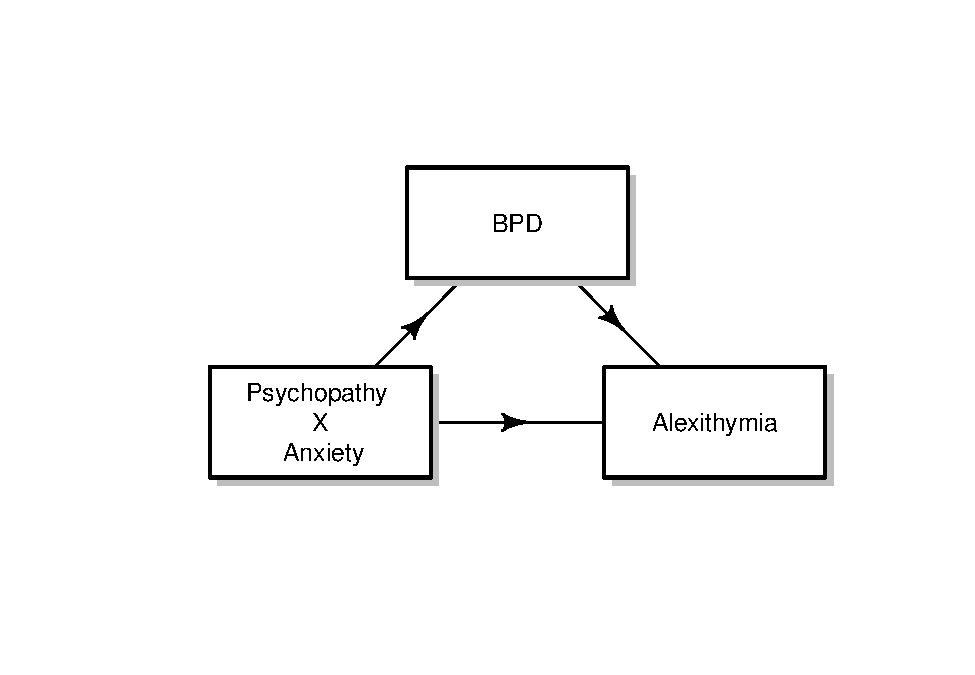
\includegraphics[width=1\linewidth]{d2m-Psychopathy_files/figure-latex/mediation-graphic-1} \caption{Mediation Graphic}\label{fig:mediation-graphic}
\end{figure}

\hypertarget{methods}{%
\section{Methods}\label{methods}}

Data were collected via structured interviews and self-report measures. The presently used assessment battery is well-validated and has been strategically refined over the past decade in forensic research (Hervé \& Yuille, 2007). We report how we determined our sample size, all data exclusions (if any), all manipulations, and all measures in the study.

\begin{table}[!htbp] \centering 
  \caption{Summary Table} 
  \label{tab:summary-table} 
\begin{tabular}{@{\extracolsep{5pt}}lccccc} 
\\[-1.8ex]\hline 
\hline \\[-1.8ex] 
Statistic & \multicolumn{1}{c}{N} & \multicolumn{1}{c}{Mean} & \multicolumn{1}{c}{St. Dev.} & \multicolumn{1}{c}{Min} & \multicolumn{1}{c}{Max} \\ 
\hline \\[-1.8ex] 
PAIBOR\_Total\_Score & 104 & 36.750 & 11.738 & 11 & 58 \\ 
PCLR\_Total\_Score\_Prorated & 104 & 23.476 & 8.070 & 4.400 & 37.000 \\ 
TAS\_Total\_Score & 104 & 49.702 & 13.852 & 20 & 82 \\ 
STAI\_Trait\_Anxiety & 104 & 45.558 & 11.213 & 23 & 72 \\ 
\hline \\[-1.8ex] 
\end{tabular} 
\end{table}

\hypertarget{participants}{%
\subsection{Participants}\label{participants}}

Collected over a four-year period, the present sample consists of 156 incarcerated females exhibiting varying levels of psychopathic and borderline tendencies. Participants range in age, from 20 to 53 (\emph{M} = 34.60, \emph{SD} = 8.78). Participants were randomly selected and subsequently informed of the nature of the study. Before screening, they were required to provide consent. Random selection was used to allow for a wide array of scores that could be systematically examined across the various facets of targeted measures.

\hypertarget{measures}{%
\subsection{Measures}\label{measures}}

\hypertarget{two-factor-psychopathy}{%
\subsubsection{Two-Factor Psychopathy}\label{two-factor-psychopathy}}

The Psychopathy Checklist---Revised (PCL---R) is a 20-item instrument operationalizing Hervey Cleckley's seminal description of sixteen characteristics that exemplify psychopathy (Cleckley, 1976; Hare, 1991). This clinical conceptualization is considered the gold standard for assessing psychopathic features in forensic samples. Both a semi-structured interview and review of institutional records comprise the assessment. Total scores may range from 0 to 40. A score of 10-19 is akin with mild psychopathy, while a score of 20-29 is illustrative of moderate psychopathy. Scores above 30 are commonly associated with severe psychopathic symptoms.

\hypertarget{borderline-personality-disorder}{%
\subsubsection{Borderline Personality Disorder}\label{borderline-personality-disorder}}

Individual dimensions of BPD were assessed using the Personality Assessment Inventory-Borderline Features scale (PAI---BOR; Morey, 1991). The PAI---BOR is a 24-item self-report measure that yields a four-factor model of BPD including affective instability, identity problems, negative relationships, and self-harm. The PAI---BOR scale has demonstrated both reliability and validity (Morey, 1991; Trull, 1995), as well as high sensitivity and specificity for individuals matching BPD criteria (Southward \& Cheavens, 2018). A score of \ldots{} is considered \ldots{}

\hypertarget{alexithymia-and-emotion}{%
\subsubsection{Alexithymia and Emotion}\label{alexithymia-and-emotion}}

The Toronto Alexithymia Scale (TAS-20; Taylor et al., 1992) is a 20-item self-report measure designed to assess facets of alexithymia across three subscales: difficulty in identifying and distinguishing feelings within oneself, difficulty in describing feelings to others, and externally oriented thinking (Karukivi \& Saarijärvi, 2014). The scale has demonstrated high internal consistency (Henry et al., 2006) and strong convergent and discriminant validity (Bagby et al., 1994). Total scores can range from 20 to 100. A score above 50 demonstrates the possibility of alexithymia, while a score above 60 illustrates strong alexithymic symptoms.

\hypertarget{exploring-dimensions-of-psychopathy}{%
\subsubsection{Exploring Dimensions of Psychopathy}\label{exploring-dimensions-of-psychopathy}}

Primary and secondary psychopathy have been shown to diverge in levels of anxiety (Vaillancourt \& Brittain, 2019). Relative to primary psychopaths, secondary psychopaths possess higher levels of trait anxiety, exhibit more borderline symptoms, and have poorer interpersonal functioning (Burns et al., 2015; Skeem et al., 2007). It is likely alexithymia diverges across the dimensions of psychopathy. In line with prior research, it is predicted that secondary psychopathy, specifically, will exhibit a relationship with alexithymia in which BPD functions as a mediator. Precedence has been established in using the interaction between psychopathy scores and STAI-Trait scores as an index of secondary psychopathy (see Lander et al., 2012; Vassileva et al., 2005). As such, the interactive term -- psychopathyXanxiety -- will be utilized in the present study. STAI-Trait scores range from 20 to 80, with higher scores being indicative of higher trait anxiety (Spielberger et al., 1970). In the literature, the assessment has shown to be a strong measure of general negative affect, as well as incorporating aspects of cognitive anxiety (Balsamo et al., 2013).

\hypertarget{procedure}{%
\subsection{Procedure}\label{procedure}}

All interviews were conducted by a clinical psychologist or trained research staff member. While incarcerated subjects are often reported as being highly reliable and compliant in psychological research (Decety et al., 2014), special ethical concerns remain for incarcerated populations as various restrictions exist on autonomy, privacy, and healthcare services. \ldots{}

\hypertarget{data-analysis}{%
\subsection{Data analysis}\label{data-analysis}}

Of the 156 total participants, 52 participants failed to complete one or more of the four assessments. Due to the heterogeneous nature of the variables, it was determined most ethical to simply remove participants who were missing data for any of the required assessments. A total of 104 participants remained for further investigation. We used various \texttt{R} packages\footnote{R (Version 4.3.2; R Core Team, 2023) and the R-packages \emph{\}citr} {[}@\}R-citr{]}, \emph{diagram} (Version 1.6.5; Soetaert, 2020), \emph{dplyr} (Version 1.1.4; Wickham, François, et al., 2023), \emph{forcats} (Version 1.0.0; Wickham, 2023a), \emph{ggformula} (Version 0.12.0; Kaplan \& Pruim, 2023), \emph{ggplot2} (Version 3.4.4; Wickham, 2016), \emph{ggsci} (Version 3.0.0; Xiao, 2023), \emph{lattice} (Version 0.21.9; Sarkar, 2008), \emph{lubridate} (Version 1.9.3; Grolemund \& Wickham, 2011), \emph{MASS} (Version 7.3.60; Venables \& Ripley, 2002), \emph{Matrix} (Version 1.6.1.1; Bates et al., 2023), \emph{mediation} (Imai, Keele, \& Yamamoto, 2010; Imai, Keele, \& Tingley, 2010; Imai et al., 2011; Imai \& Yamamoto, 2013; Version 4.5.0; Tingley et al., 2014), \emph{mosaic} (Version 1.9.0; Pruim et al., 2017, 2023), \emph{mosaicData} (Version 0.20.4; Pruim et al., 2023), \emph{mvtnorm} (Version 1.2.4; Genz \& Bretz, 2009), \emph{papaja} (Version 0.1.1.9001; Aust \& Barth, 2022), \emph{psych} (Version 2.4.1; William Revelle, 2024), \emph{purrr} (Version 1.0.2; Wickham \& Henry, 2023), \emph{readr} (Version 2.1.4; Wickham, Hester, et al., 2023), \emph{sandwich} (Zeileis, 2004, 2006; Version 3.1.0; Zeileis et al., 2020), \emph{shape} (Version 1.4.6; Soetaert, 2021), \emph{shiny} (Version 1.8.0; Chang et al., 2023), \emph{stargazer} (Version 5.2.3; Hlavac, 2022), \emph{stringr} (Version 1.5.1; Wickham, 2023b), \emph{tibble} (Version 3.2.1; Müller \& Wickham, 2023), \emph{tidyr} (Version 1.3.1; Wickham et al., 2024), \emph{tidyverse} (Version 2.0.0; Wickham et al., 2019), and \emph{tinylabels} (Version 0.2.4; Barth, 2023)} for all our analyses.

\hypertarget{results}{%
\section{Results}\label{results}}

Descriptive statistics for the assessments of interest can be seen in Table~\ref{tab:summary-table}.



\begin{verbatim}
## Warning: Removed 2 rows containing missing values (`geom_bar()`).
\end{verbatim}

\begin{figure}
\centering
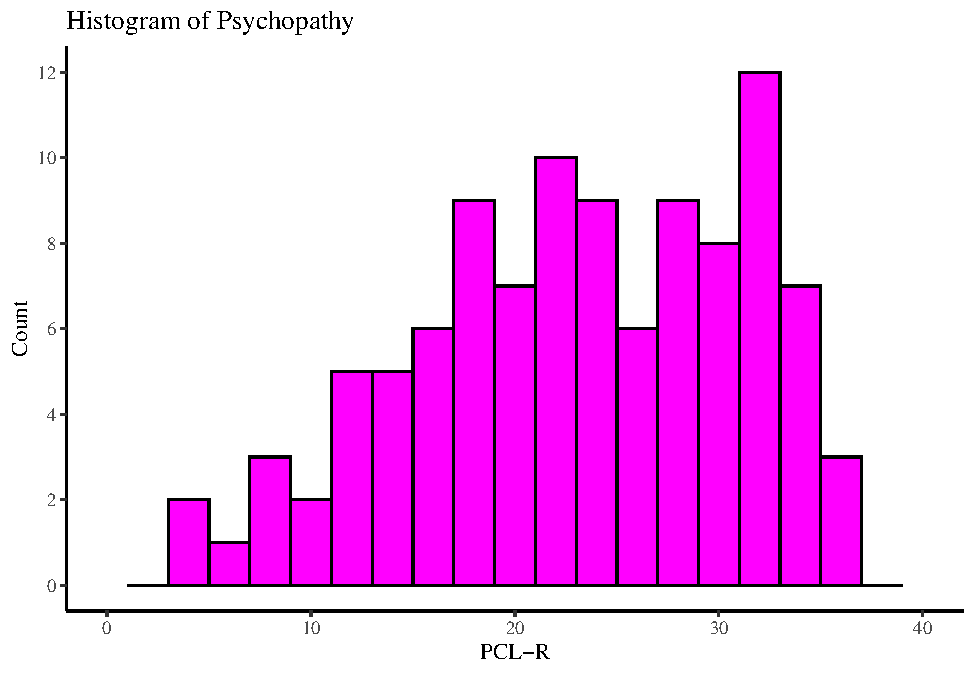
\includegraphics{d2m-Psychopathy_files/figure-latex/PCLR-descriptives-1.pdf}
\caption{\label{fig:PCLR-descriptives}Histogram of score distribution on the PCL--R.}
\end{figure}

As seen in Figure~\ref{fig:PCLR-descriptives}, our distribution of PCL--R scores is left-skewed, with more participants falling on the higher end of the spectrum. This is ?consistent? with past studies conducted with incarcerated populations (probably Decety). Other score assessment distributions can be found in the appendix.

\begin{verbatim}
## Warning: Removed 2 rows containing missing values (`geom_bar()`).
\end{verbatim}

\begin{verbatim}
## Warning: Removed 1 rows containing missing values (`geom_bar()`).
\end{verbatim}

\begin{verbatim}
## Warning: Removed 1 rows containing non-finite values (`stat_bin()`).
\end{verbatim}

\begin{verbatim}
## Warning: Removed 2 rows containing missing values (`geom_bar()`).
\end{verbatim}



\begin{figure}
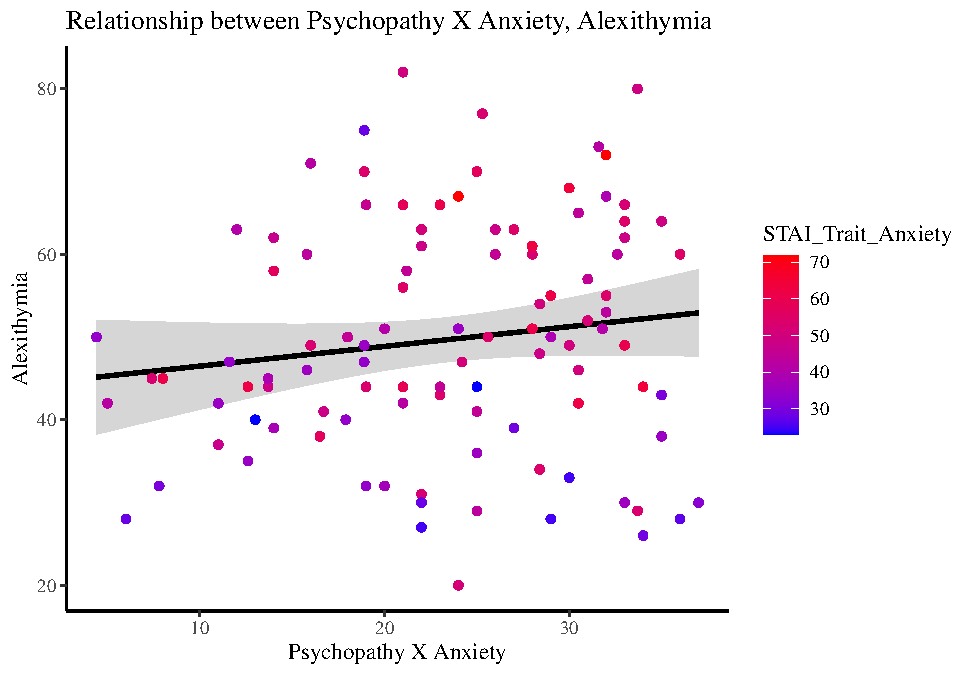
\includegraphics[width=1\linewidth]{d2m-Psychopathy_files/figure-latex/c-path-scatterplot-1} \caption{Scatterplot demonstrating relationship between the interactive term of psychopathy and trait anxiety with alexithymia in our sample of incarcerated women.}\label{fig:c-path-scatterplot}
\end{figure}

Figure~\ref{fig:c-path-scatterplot} shows a moderate correlation of 0.37 between PsychopathyXAnxiety and Alexithymia. \ldots talk about colors



\begin{figure}
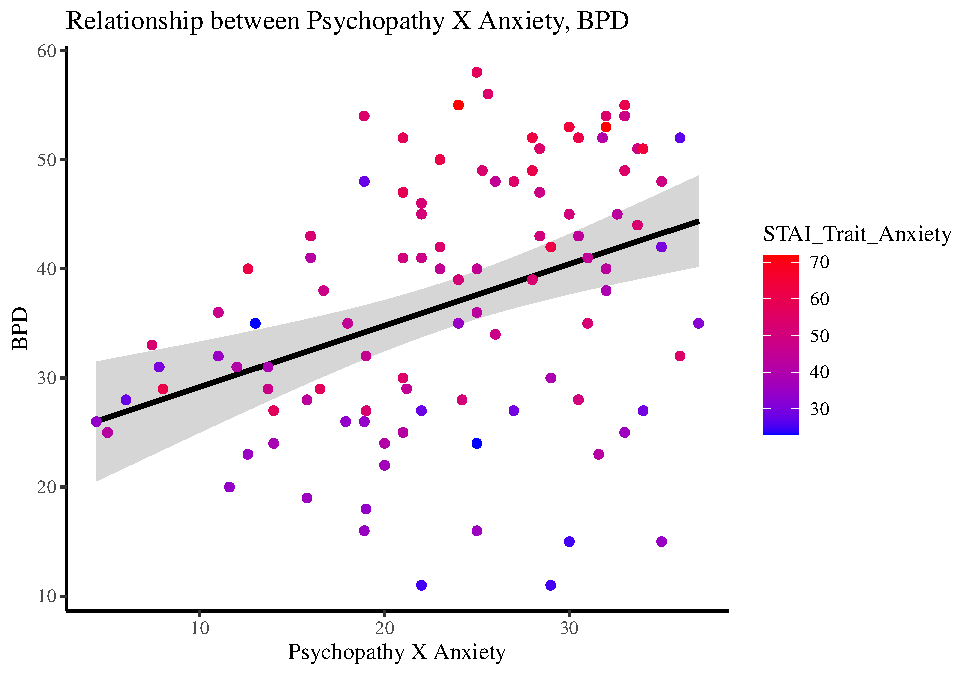
\includegraphics[width=1\linewidth]{d2m-Psychopathy_files/figure-latex/a-path-scatterplot-1} \caption{Scatterplot demonstrating relationship between the interactive term of psychopathy and trait anxiety with borderline personality disorder in our sample of incarcerated women.}\label{fig:a-path-scatterplot}
\end{figure}

Figure~\ref{fig:a-path-scatterplot} shows a moderate to strong correlation of 0.66 between PsychopathyXAnxiety and BPD. \ldots talk about colors

All assessment scores (including the interactive term) were standardized. Mediation analyses with bootstrapping were conducted to test the primary hypothesis. Unlike other methods, bootstrapping is not limited by the assumption of normality. The interaction term of PCL--R Total Score and STAI Trait Anxiety was entered as the predictor, and PAI-BOR Total Score was entered as the mediating term. Total Score on the TAS was our outcome variable. A significant Average Causal Mediation Effect (ACME) would demonstrate support of our hypothesis.

In order to run a mediation analysis, one must ensure significant relationships exist between predictor and outcome, predictor and mediator, and mediator and outcome. The present data support these requirements, thus we were able to proceed with our mediation analysis. Results for these preliminary analyses can be seen in Table~\ref{tab:prelim-regression-output} of the Appendix.

\begin{table}[!htbp] \centering 
  \caption{Simple Linear Regression Results} 
  \label{tab:simple-regression-output} 
\begin{tabular}{@{\extracolsep{1pt}}lcccc} 
\\[-1.8ex]\hline 
\hline \\[-1.8ex] 
 & \multicolumn{4}{c}{\textit{Dependent variable:}} \\ 
\cline{2-5} 
\\[-1.8ex] & TAS Total & Factor 1 & Factor 2 & Factor 3 \\ 
\\[-1.8ex] & (1) & (2) & (3) & (4)\\ 
\hline \\[-1.8ex] 
 PsychopathyXAnxiety & 0.373$^{***}$ & 0.418$^{***}$ & 0.291$^{***}$ & 0.197$^{**}$ \\ 
  & (0.092) & (0.090) & (0.095) & (0.097) \\ 
  & & & & \\ 
 Constant & $-$0.000 & $-$0.000 & $-$0.000 & 0.000 \\ 
  & (0.091) & (0.090) & (0.094) & (0.097) \\ 
  & & & & \\ 
\hline \\[-1.8ex] 
Observations & 104 & 104 & 104 & 104 \\ 
R$^{2}$ & 0.139 & 0.174 & 0.085 & 0.039 \\ 
Adjusted R$^{2}$ & 0.131 & 0.166 & 0.076 & 0.030 \\ 
Residual Std. Error (df = 102) & 0.932 & 0.913 & 0.961 & 0.985 \\ 
F Statistic (df = 1; 102) & 16.501$^{***}$ & 21.551$^{***}$ & 9.463$^{***}$ & 4.140$^{**}$ \\ 
\hline 
\hline \\[-1.8ex] 
\textit{Note:}  & \multicolumn{4}{r}{$^{*}$p$<$0.1; $^{**}$p$<$0.05; $^{***}$p$<$0.01} \\ 
\end{tabular} 
\end{table}

\begin{table}[!htbp] \centering 
  \caption{Multiple Linear Regression Results} 
  \label{tab:mult-regression-output} 
\begin{tabular}{@{\extracolsep{1pt}}lcccc} 
\\[-1.8ex]\hline 
\hline \\[-1.8ex] 
 & \multicolumn{4}{c}{\textit{Dependent variable:}} \\ 
\cline{2-5} 
\\[-1.8ex] & TAS Total & Factor 1 & Factor 2 & Factor 3 \\ 
\\[-1.8ex] & (1) & (2) & (3) & (4)\\ 
\hline \\[-1.8ex] 
 PsychopathyXAnxiety & 0.111 & 0.096 & 0.036 & 0.154 \\ 
  & (0.116) & (0.110) & (0.121) & (0.130) \\ 
  & & & & \\ 
 BPD & 0.398$^{***}$ & 0.487$^{***}$ & 0.386$^{***}$ & 0.066 \\ 
  & (0.116) & (0.110) & (0.121) & (0.130) \\ 
  & & & & \\ 
 Constant & $-$0.000 & $-$0.000 & $-$0.000 & 0.000 \\ 
  & (0.087) & (0.082) & (0.090) & (0.097) \\ 
  & & & & \\ 
\hline \\[-1.8ex] 
Observations & 104 & 104 & 104 & 104 \\ 
R$^{2}$ & 0.228 & 0.308 & 0.169 & 0.041 \\ 
Adjusted R$^{2}$ & 0.213 & 0.294 & 0.153 & 0.022 \\ 
Residual Std. Error (df = 101) & 0.887 & 0.840 & 0.921 & 0.989 \\ 
F Statistic (df = 2; 101) & 14.949$^{***}$ & 22.477$^{***}$ & 10.273$^{***}$ & 2.182 \\ 
\hline 
\hline \\[-1.8ex] 
\textit{Note:}  & \multicolumn{4}{r}{$^{*}$p$<$0.1; $^{**}$p$<$0.05; $^{***}$p$<$0.01} \\ 
\end{tabular} 
\end{table}

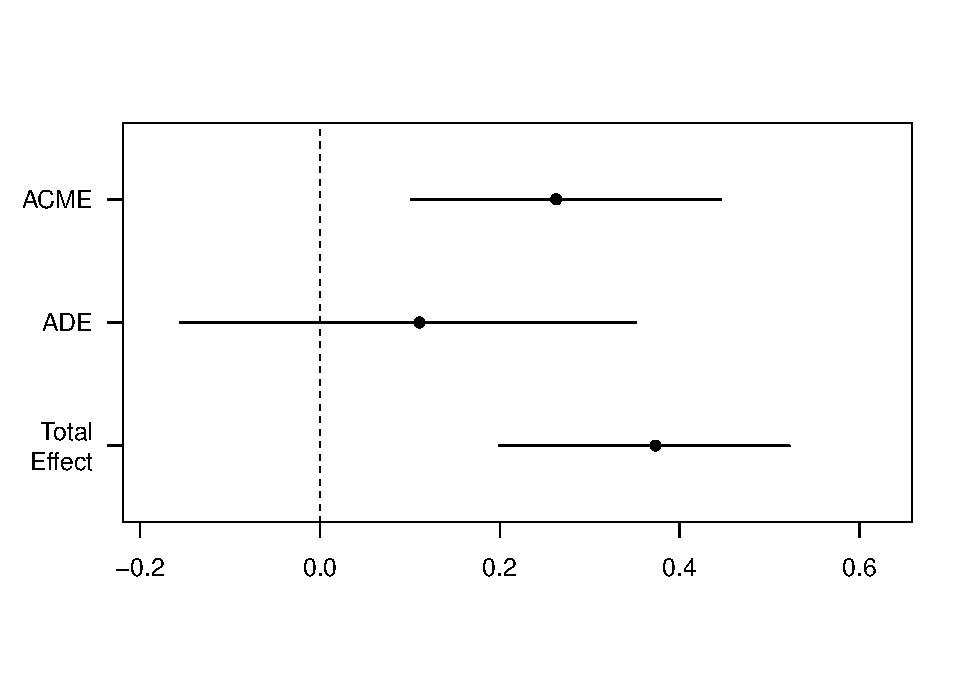
\includegraphics{d2m-Psychopathy_files/figure-latex/ugly-plots-1.pdf} 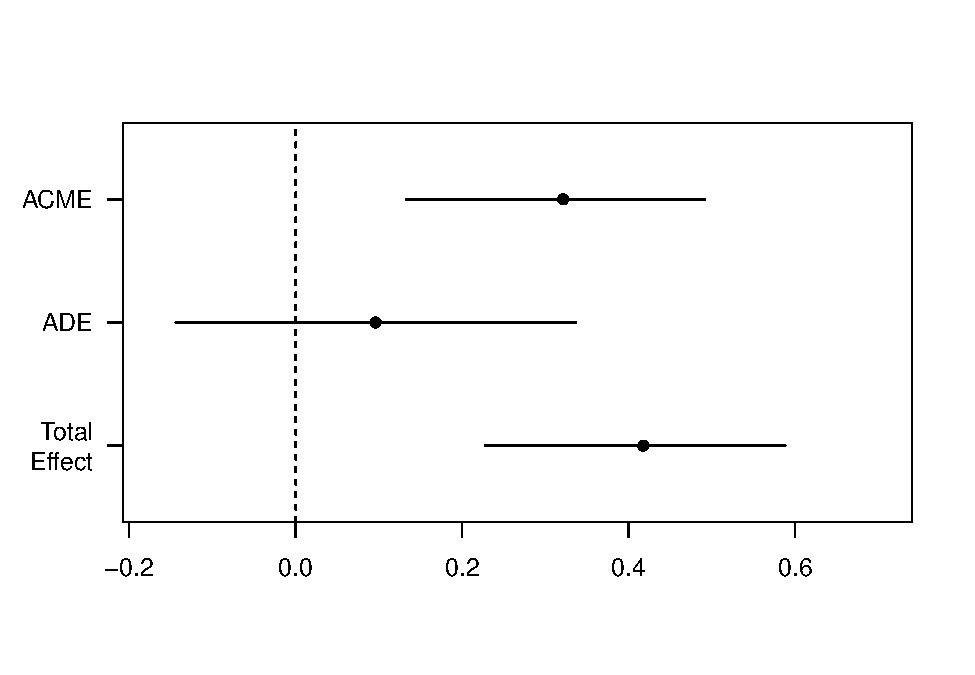
\includegraphics{d2m-Psychopathy_files/figure-latex/ugly-plots-2.pdf} 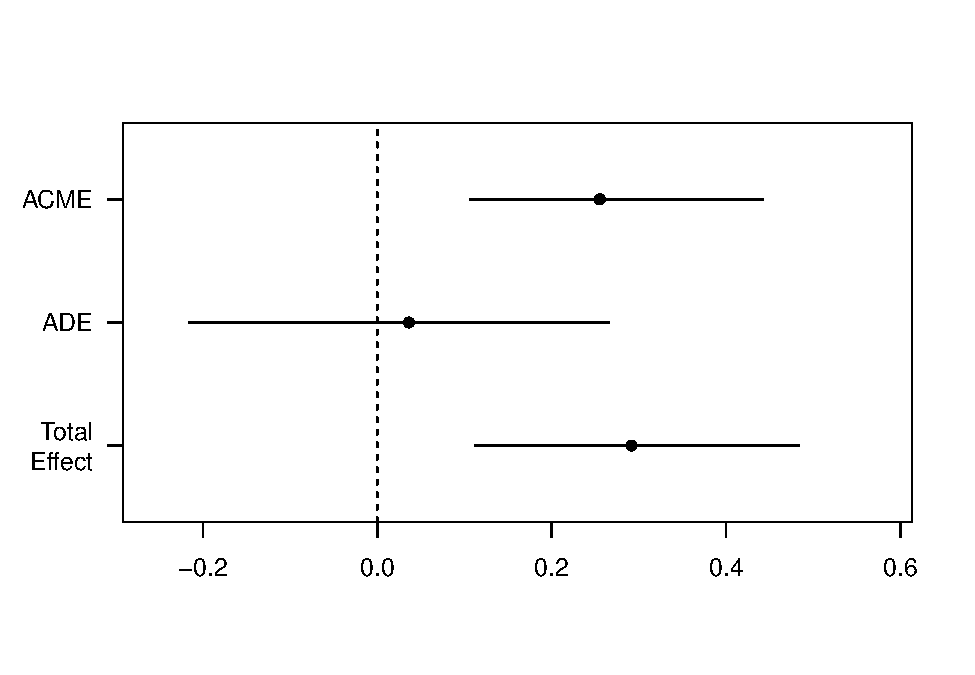
\includegraphics{d2m-Psychopathy_files/figure-latex/ugly-plots-3.pdf} 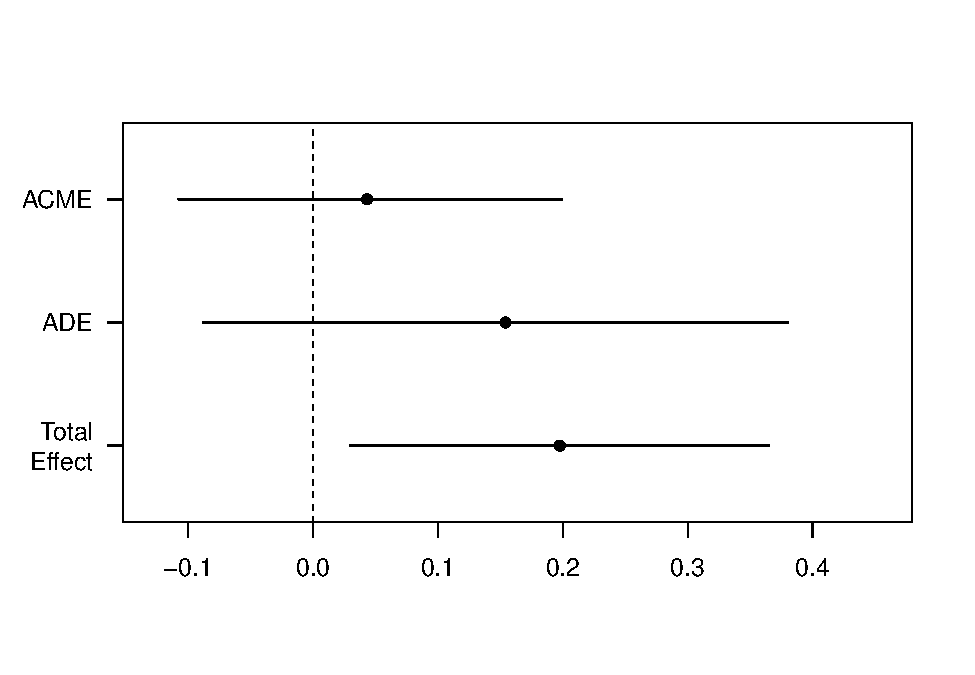
\includegraphics{d2m-Psychopathy_files/figure-latex/ugly-plots-4.pdf}

\emph{reference tables 2 and 3} There is a significant relationship between predictor and outcome (\emph{p} \textless{} .001). However, this effect goes away when adding BPD as a mediator (\emph{p} = ). This suggests that the presence of BPD acts as a mechanism through which the predictor influences the outcome. The significant, full mediation effect we observed suggests that a portion of the total effect of the predictor on the outcome is explained by the mediator (\emph{p} = ).

Three subfactors defined in the TAS are believed to compose alexithymia: difficulty identifying feelings (Factor 1), difficulty describing feelings (Factor 2), and externally-oriented thinking (Factor 3). As we collected subfactor scores for every participant, an exploratory analysis could be conducted to get a sense of what specific parts of emotional processing psychopathy and BPD may be impacting. We found that, replacing the total TAS score for Factor 1 and Factor 2, the significant mediation effect remained in tact. However, designating Factor 3 as an outcome left us with an insignificant model. The change in significant effect when replacing for specific factors of TAS suggests the mediation effect may depend on specific aspects or dimensions of alexithymia. It is critical these results are analyzed with caution as no hypotheses regarding TAS subfactors were determined \emph{a priori} and the theoretical lineage is at present quite limited.

\hypertarget{discussion}{%
\section{Discussion}\label{discussion}}

The results of the current study further advocate a promising role for borderline personality disorder in the relationship between psychopathy and alexithymia among women. Consistent with prior research, BPD was found to have a significant mediation effect on the association between an index of secondary psychopathy and alexithymia. However, contrary to previous findings, the inclusion of BPD fully accounted for this relationship. This is evidenced by the lack of a significant direct relationship between psychopathy and alexithymia after the inclusion of BPD.

There are a few possible explanations for this finding. No study, to our knowledge, has utilized the exact same assessment battery when addressing these specific questions. While popular assessments are likely well-validated and replicable, it is possible subtly distinct indicators are being captured in each set of evaluations.

Prior research inspiring this study was conducted primarily on low-psychopathy, community-based samples (Lander et al., 2012; Ridings \& Lutz-Zois, 2014). It is certainly possible divergences exist between the presentation of psychopathy and BPD in incarcerated versus non-incarcerated populations. We already know that both psychopathy and BPD are much more prevalent within the prison system (Barbara Burton \& Fabian M. Saleh, 2020; Conn et al., 2010). However, little is known with regards to the relationship between psychopathy and BPD in women as it's compared across unique settings. Future research may wish to flesh out these nuances explicitly.

Regarding the findings from our exploratory analyses, it is possible that BPD symptoms uniquely impact certain dimensions of alexithymia as operationalized by the TAS-20. When considering what each of the three factors represent, it may be plausible that BPD would affect factors 1 and 2 -- addressing emotional comprehension and recognition -- and not 3 -- externally-oriented thinking -- as BPD may be more closely associated with internalizing features (Beauchaine et al., 2009). More research that addresses the role of both psychopathy and BPD on externally-oriented thinking is required here to draw firmer conclusions. Additionally, as these hypotheses were not established \emph{a priori}, studies replicating discoveries here are warranted.

Additional factors and moderators merit further exploration. Other relevant comorbidities -- such as PTSD -- may influence the mediation pathway seen here in a way that could further explicate these nuanced relationships. Beyond this, we would like to strongly advocate for future research to conduct factor analyses that break down BPD further in order to understand what specific mechanisms of the disorder might be at play in this relationship. According to the DSM-\emph{V}, BPD can be diagnosed through 256 unique combinations (cite dsm?). This statistic alone highlights the severe phenomenological heterogeneity at play with regards to this personality disorder. It is critical studies continue to amplify attention here -- possibly with regards to dimensionalities, unique etiologies, or other unconsidered clinical factors at play -- to avoid BPD acting as a diagnostic `catch-all' for emotion dysregulation or maladaptive social behavior.

BPD, as with all personality disorders, have ``cultural histories'' (Bjorklund, 2006, p. 3). Sociocultural factors will inevitably play a role in disease and diagnostic conditions, yet this hardly explains why a BPD diagnosis is considerably more common in women than in men. More research should more deeply and centrally seek to elucidate what many actually be contributing to diagnostic disparity when it comes to gender and what may simply be a product of bias. It continues to remain possible that ASPD and BPD are simply gender-based constructions of arriving at the same end point (Beauchaine et al., 2009). On a grander scale, gender is not the only means for demonstrating diversity in psychopathological manifestation. Future research should consider other means of distinguishing psychopathy as well.

The curious diversity of this mediation effect is certainly cause for future research. Emotion expression and regulation play crucial roles in daily interactions and interpersonal relationships. It is evident that abnormal emotional processing is central to both psychopathy and BPD. As such, research into this area will help to tailor essential treatment that elucidates earlier intervention points for how and when this concoction of maladaptive processes may contribute to an endgame of incarceration. This information can guide the development of targeted interventions or strategies based on specific factors that are most influenced by the mediation process. Dialectical Behavioral Therapy (DBT; Linehan et al., 1993) and DBT-inspired treatments have demonstrated preliminary yet promising results for incarcerated female populations (Per et al., 2020). Regardless, these changes in significance emphasize the need for careful and nuanced interpretation, taking into account the specific characteristics and dynamics at play for each factor within the composite variables.

We do not doubt that the relationship between psychopathy, anxiety, BPD, and alexithymia is multifaceted and complex. Nevertheless, the presence of distress and emotional dysregulation is exceptionally embodied for the people inflicted; it remains critical to continue research to help not only understand these mechanisms, but also to inform tailored treatment that is less costly, more effective, and deterrent of negative psychopathic behavior.

Presenting findings on a unique population such as this one requires cautious interpretation. While we are intrigued by the prospects suggested here, we are limited in our ability to generalize conclusions drawn. That being said, we are hopeful that this study brings us one step closer to obtaining a clearer, more concise picture of psychopathy as it manifests in women.

\newpage

\hypertarget{references}{%
\section{References}\label{references}}

\hypertarget{refs}{}
\begin{CSLReferences}{1}{0}
\leavevmode\vadjust pre{\hypertarget{ref-R-papaja}{}}%
Aust, F., \& Barth, M. (2022). \emph{{papaja}: {Prepare} reproducible {APA} journal articles with {R Markdown}}. \url{https://github.com/crsh/papaja}

\leavevmode\vadjust pre{\hypertarget{ref-bagbyTwentyitemTorontoAlexithymia1994}{}}%
Bagby, R. M., Taylor, G. J., \& Parker, J. D. A. (1994). The twenty-item {Toronto Alexithymia} scale---{II}. {Convergent}, discriminant, and concurrent validity. \emph{Journal of Psychosomatic Research}, \emph{38}(1), 33--40. \url{https://doi.org/10.1016/0022-3999(94)90006-X}

\leavevmode\vadjust pre{\hypertarget{ref-balsamoStateTraitAnxietyInventory2013}{}}%
Balsamo, M., Romanelli, R., Innamorati, M., Ciccarese, G., Carlucci, L., \& Saggino, A. (2013). The {State-Trait Anxiety Inventory}: {Shadows} and {Lights} on its {Construct Validity}. \emph{Journal of Psychopathology and Behavioral Assessment}, \emph{35}(4), 475--486. \url{https://doi.org/10.1007/s10862-013-9354-5}

\leavevmode\vadjust pre{\hypertarget{ref-barbaraburtonPsychopathyInsightsGeneral2020}{}}%
Barbara Burton, M. D., \& Fabian M. Saleh, M. D. (2020). \emph{Psychopathy: {Insights} for {General Practice}}. \emph{37}.

\leavevmode\vadjust pre{\hypertarget{ref-R-tinylabels}{}}%
Barth, M. (2023). \emph{{tinylabels}: Lightweight variable labels}. \url{https://cran.r-project.org/package=tinylabels}

\leavevmode\vadjust pre{\hypertarget{ref-R-Matrix}{}}%
Bates, D., Maechler, M., \& Jagan, M. (2023). \emph{Matrix: Sparse and dense matrix classes and methods}. \url{https://CRAN.R-project.org/package=Matrix}

\leavevmode\vadjust pre{\hypertarget{ref-beauchaineMultifinalityDevelopmentPersonality2009}{}}%
Beauchaine, T. P., Klein, D. N., Crowell, S. E., Derbidge, C., \& Gatzke-Kopp, L. (2009). Multifinality in the development of personality disorders: {A Biology} {\texttimes} {Sex} {\texttimes} {Environment} interaction model of antisocial and borderline traits. \emph{Development and Psychopathology}, \emph{21}(3), 735--770. \url{https://doi.org/10.1017/S0954579409000418}

\leavevmode\vadjust pre{\hypertarget{ref-bjorklundNOMANLAND2006}{}}%
Bjorklund, P. (2006). {NO MAN}'{S LAND}: {GENDER BIAS AND SOCIAL CONSTRUCTIVISM IN THE DIAGNOSIS OF BORDERLINE PERSONALITY DISORDER}. \emph{Issues in Mental Health Nursing}, \emph{27}(1), 3--23. \url{https://doi.org/10.1080/01612840500312753}

\leavevmode\vadjust pre{\hypertarget{ref-burnsEvaluatingEmotionProcessing2015}{}}%
Burns, S., Roberts, L. D., Egan, S., \& Kane, R. (2015). Evaluating emotion processing and trait anxiety as predictors of non-criminal psychopathy. \emph{Personality and Individual Differences}, \emph{81}, 148--154. \url{https://doi.org/10.1016/j.paid.2014.08.044}

\leavevmode\vadjust pre{\hypertarget{ref-R-shiny}{}}%
Chang, W., Cheng, J., Allaire, J., Sievert, C., Schloerke, B., Xie, Y., Allen, J., McPherson, J., Dipert, A., \& Borges, B. (2023). \emph{Shiny: Web application framework for r}. \url{https://CRAN.R-project.org/package=shiny}

\leavevmode\vadjust pre{\hypertarget{ref-clarkinDefiningMechanismsBorderline2005}{}}%
Clarkin, J. F., \& Posner, M. (2005). Defining the {Mechanisms} of {Borderline Personality Disorder}. \emph{Psychopathology}, \emph{38}(2), 56--63. \url{https://doi.org/10.1159/000084812}

\leavevmode\vadjust pre{\hypertarget{ref-cleckleyMaskSanityAttempt1976}{}}%
Cleckley, H. M. (1976). \emph{The mask of sanity: An attempt to clarify some issues about the so-called psychopathic personality} (5th ed). {Mosby}.

\leavevmode\vadjust pre{\hypertarget{ref-connBorderlinePersonalityDisorder2010}{}}%
Conn, C., Warden, R., Stuewig, J., Kim, E. H., Harty, L., Hastings, M., \& Tangney, J. P. (2010). \href{https://www.ncbi.nlm.nih.gov/pmc/articles/PMC4825675}{Borderline {Personality Disorder Among Jail Inmates}: {How Common} and {How Distinct}?} \emph{Corrections Compendium}, \emph{35}(4), 6--13.

\leavevmode\vadjust pre{\hypertarget{ref-debritoPsychopathy2021}{}}%
De Brito, S. A., Forth, A. E., Baskin-Sommers, A. R., Brazil, I. A., Kimonis, E. R., Pardini, D., Frick, P. J., Blair, R. J. R., \& Viding, E. (2021). Psychopathy. \emph{Nature Reviews Disease Primers}, \emph{7}(1), 1--21. \url{https://doi.org/10.1038/s41572-021-00282-1}

\leavevmode\vadjust pre{\hypertarget{ref-devogelGenderDifferencesAssessment2016}{}}%
De Vogel, V., \& Lancel, M. (2016). Gender {Differences} in the {Assessment} and {Manifestation} of {Psychopathy}: {Results From} a {Multicenter Study} in {Forensic Psychiatric Patients}. \emph{International Journal of Forensic Mental Health}, \emph{15}(1), 97--110. \url{https://doi.org/10.1080/14999013.2016.1138173}

\leavevmode\vadjust pre{\hypertarget{ref-decetyNeuralProcessingDynamic2014}{}}%
Decety, J., Skelly, L., Yoder, K. J., \& Kiehl, K. A. (2014). Neural processing of dynamic emotional facial expressions in psychopaths. \emph{Social Neuroscience}, \emph{9}(1), 36--49. \url{https://doi.org/10.1080/17470919.2013.866905}

\leavevmode\vadjust pre{\hypertarget{ref-effersonExaminingGenderDifferences2018}{}}%
Efferson, L. M., \& Glenn, A. L. (2018). Examining gender differences in the correlates of psychopathy: {A} systematic review of emotional, cognitive, and morality-related constructs. \emph{Aggression and Violent Behavior}, \emph{41}, 48--61. \url{https://doi.org/10.1016/j.avb.2018.05.009}

\leavevmode\vadjust pre{\hypertarget{ref-R-mvtnorm}{}}%
Genz, A., \& Bretz, F. (2009). \emph{Computation of multivariate normal and t probabilities}. Springer-Verlag.

\leavevmode\vadjust pre{\hypertarget{ref-goerlichMultifacetedNatureAlexithymia2018}{}}%
Goerlich, K. S. (2018). The {Multifaceted Nature} of {Alexithymia} -- {A Neuroscientific Perspective}. \emph{Frontiers in Psychology}, \emph{9}, 1614. \url{https://doi.org/10.3389/fpsyg.2018.01614}

\leavevmode\vadjust pre{\hypertarget{ref-R-lubridate}{}}%
Grolemund, G., \& Wickham, H. (2011). Dates and times made easy with {lubridate}. \emph{Journal of Statistical Software}, \emph{40}(3), 1--25. \url{https://www.jstatsoft.org/v40/i03/}

\leavevmode\vadjust pre{\hypertarget{ref-hareManualHarePsychopathy}{}}%
Hare, R. D. (1991). \emph{Manual for the {Hare Psychopathy Checklist-Revised}}. {Toronto: Multi-Health Systems}.

\leavevmode\vadjust pre{\hypertarget{ref-hare2003psychopathy}{}}%
Hare, R. D. (2003). Psychopathy checklist---revised. \emph{Psychological Assessment}.

\leavevmode\vadjust pre{\hypertarget{ref-henryCognitivePsychosocialCorrelates2006}{}}%
Henry, J. D., Phillips, L. H., Crawford, J. R., Theodorou, G., \& Summers, F. (2006). Cognitive and psychosocial correlates of alexithymia following traumatic brain injury. \emph{Neuropsychologia}, \emph{44}(1), 62--72. \url{https://doi.org/10.1016/j.neuropsychologia.2005.04.011}

\leavevmode\vadjust pre{\hypertarget{ref-hervePsychopathTheoryResearch2007}{}}%
Hervé, H., \& Yuille, J. C. (Eds.). (2007). \emph{The psychopath: Theory, research, and practice}. {Lawrence Erlbaum Associates}.

\leavevmode\vadjust pre{\hypertarget{ref-R-stargazer}{}}%
Hlavac, M. (2022). \emph{Stargazer: Well-formatted regression and summary statistics tables}. Social Policy Institute. \url{https://CRAN.R-project.org/package=stargazer}

\leavevmode\vadjust pre{\hypertarget{ref-huntGeneticEnvironmentalOverlap2015}{}}%
Hunt, E., Bornovalova, M. A., \& Patrick, C. J. (2015). Genetic and environmental overlap between borderline personality disorder traits and psychopathy: Evidence for promotive effects of factor 2 and protective effects of factor 1. \emph{Psychological Medicine}, \emph{45}(7), 1471--1481. \url{https://doi.org/10.1017/S0033291714002608}

\leavevmode\vadjust pre{\hypertarget{ref-R-mediation_c}{}}%
Imai, K., Keele, L., \& Tingley, D. (2010). A general approach to causal mediation analysis. \emph{Psychological Methods}, \emph{15}(4), 309--334. \url{http://imai.princeton.edu/research/BaronKenny.html}

\leavevmode\vadjust pre{\hypertarget{ref-R-mediation_d}{}}%
Imai, K., Keele, L., Tingley, D., \& Yamamoto, T. (2011). Unpacking the black box of causality: Learning about causal mechanisms from experimental and observational studies. \emph{American Political Science Review}, \emph{105}(4), 765--789. \url{http://imai.princeton.edu/research/mediationP.html}

\leavevmode\vadjust pre{\hypertarget{ref-R-mediation_b}{}}%
Imai, K., Keele, L., \& Yamamoto, T. (2010). Identification, inference, and sensitivity analysis for causal mediation effects. \emph{Statistical Science}, \emph{25}(1), 51--71. \url{http://imai.princeton.edu/research/mediation.html}

\leavevmode\vadjust pre{\hypertarget{ref-R-mediation_e}{}}%
Imai, K., \& Yamamoto, T. (2013). Identification and sensitivity analysis for multiple causal mechanisms: Revisiting evidence from framing experiments. \emph{Political Analysis}, \emph{21}(2), 141--171. \url{http://imai.princeton.edu/research/medsens.html}

\leavevmode\vadjust pre{\hypertarget{ref-R-ggformula}{}}%
Kaplan, D., \& Pruim, R. (2023). \emph{Ggformula: Formula interface to the grammar of graphics}. \url{https://CRAN.R-project.org/package=ggformula}

\leavevmode\vadjust pre{\hypertarget{ref-karpmanNeedSeparatingPsychopathy1941}{}}%
Karpman, B. (1941). On the need of separating psychopathy into two distinct clinical types: The symptomatic and the idiopathic. \emph{Journal of Criminal Psychopathology}, \emph{3}, 112--137.

\leavevmode\vadjust pre{\hypertarget{ref-karukiviDevelopmentAlexithymicPersonality2014}{}}%
Karukivi, M., \& Saarijärvi, S. (2014). Development of alexithymic personality features. \emph{World Journal of Psychiatry}, \emph{4}(4), 91. \url{https://doi.org/10.5498/wjp.v4.i4.91}

\leavevmode\vadjust pre{\hypertarget{ref-landerDifferentialAssociationAlexithymia2012}{}}%
Lander, G. C., Lutz-Zois, C. J., Rye, M. S., \& Goodnight, J. A. (2012). The differential association between alexithymia and primary versus secondary psychopathy. \emph{Personality and Individual Differences}, \emph{52}(1), 45--50. \url{https://doi.org/10.1016/j.paid.2011.08.027}

\leavevmode\vadjust pre{\hypertarget{ref-linehan1993dialectical}{}}%
Linehan, M. M., Heard, H., Clarkin, J., Marziali, E., \& Munroe-Blum, H. (1993). Dialectical behavior therapy for borderline personality disorder. \emph{New York: Guilford}.

\leavevmode\vadjust pre{\hypertarget{ref-morey1991personality}{}}%
Morey, L. C. (1991). \emph{Personality assessment inventory}. Psychological Assessment Resources Odessa, FL.

\leavevmode\vadjust pre{\hypertarget{ref-R-tibble}{}}%
Müller, K., \& Wickham, H. (2023). \emph{Tibble: Simple data frames}. \url{https://CRAN.R-project.org/package=tibble}

\leavevmode\vadjust pre{\hypertarget{ref-nationalinstituteofmentalhealthBorderlinePersonalityDisorder2023}{}}%
National Institute of Mental Health. (2023). Borderline {Personality Disorder}. In \emph{U.S. Department of Health and Human Services, National Institutes of Health}.

\leavevmode\vadjust pre{\hypertarget{ref-newhillPsychopathyScoresReveal2010}{}}%
Newhill, C. E., Vaughn, M. G., \& DeLisi, M. (2010). Psychopathy scores reveal heterogeneity among patients with borderline personality disorder. \emph{Journal of Forensic Psychiatry \& Psychology}, \emph{21}(2), 202--220. \url{https://doi.org/10.1080/14789940903281157}

\leavevmode\vadjust pre{\hypertarget{ref-perEvaluatingEffectivenessMindfulnessBased2020}{}}%
Per, M., Spinelli, C., Sadowski, I., Schmelefske, E., Anand, L., \& Khoury, B. (2020). Evaluating the {Effectiveness} of {Mindfulness-Based Interventions} in {Incarcerated Populations}: {A Meta-Analysis}. \emph{Criminal Justice and Behavior}, \emph{47}(3), 310--330. \url{https://doi.org/10.1177/0093854819891457}

\leavevmode\vadjust pre{\hypertarget{ref-R-mosaic}{}}%
Pruim, R., Kaplan, D. T., \& Horton, N. J. (2017). The mosaic package: Helping students to 'think with data' using r. \emph{The R Journal}, \emph{9}(1), 77--102. \url{https://journal.r-project.org/archive/2017/RJ-2017-024/index.html}

\leavevmode\vadjust pre{\hypertarget{ref-R-mosaicData}{}}%
Pruim, R., Kaplan, D., \& Horton, N. (2023). \emph{mosaicData: Project MOSAIC data sets}. \url{https://CRAN.R-project.org/package=mosaicData}

\leavevmode\vadjust pre{\hypertarget{ref-R-base}{}}%
R Core Team. (2023). \emph{R: A language and environment for statistical computing}. R Foundation for Statistical Computing. \url{https://www.R-project.org/}

\leavevmode\vadjust pre{\hypertarget{ref-ridingsEmotionalDysregulationBorderline2014}{}}%
Ridings, L. E., \& Lutz-Zois, C. J. (2014). Emotional dysregulation and {Borderline Personality Disorder}: {Explaining} the link between secondary psychopathy and alexithymia. \emph{Personality and Individual Differences}, \emph{57}, 14--19. \url{https://doi.org/10.1016/j.paid.2013.09.008}

\leavevmode\vadjust pre{\hypertarget{ref-rutherfordGenderDifferencesRelationship1998}{}}%
Rutherford, M. J., Alterman, A. I., Cacciola, J. S., \& McKay, J. R. (1998). Gender {Differences} in the {Relationship} of {Antisocial Personality Disorder Criteria} to {Psychopathy Checklist-Revised Scores}. \emph{Journal of Personality Disorders}, \emph{12}(1), 69--76. \url{https://doi.org/10.1521/pedi.1998.12.1.69}

\leavevmode\vadjust pre{\hypertarget{ref-R-lattice}{}}%
Sarkar, D. (2008). \emph{Lattice: Multivariate data visualization with r}. Springer. \url{http://lmdvr.r-forge.r-project.org}

\leavevmode\vadjust pre{\hypertarget{ref-sellbomClassificationPsychopathy2021}{}}%
Sellbom, M., \& Drislane, L. E. (2021). The classification of psychopathy. \emph{Aggression and Violent Behavior}, \emph{59}, 101473. \url{https://doi.org/10.1016/j.avb.2020.101473}

\leavevmode\vadjust pre{\hypertarget{ref-skeemTwoSubtypesPsychopathic2007}{}}%
Skeem, J., Johansson, P., Andershed, H., Kerr, M., \& Louden, J. E. (2007). Two subtypes of psychopathic violent offenders that parallel primary and secondary variants. \emph{Journal of Abnormal Psychology}, \emph{116}(2), 395--409. \url{https://doi.org/10.1037/0021-843X.116.2.395}

\leavevmode\vadjust pre{\hypertarget{ref-R-diagram}{}}%
Soetaert, K. (2020). \emph{Diagram: Functions for visualising simple graphs (networks), plotting flow diagrams}. \url{https://CRAN.R-project.org/package=diagram}

\leavevmode\vadjust pre{\hypertarget{ref-R-shape}{}}%
Soetaert, K. (2021). \emph{Shape: Functions for plotting graphical shapes, colors}. \url{https://CRAN.R-project.org/package=shape}

\leavevmode\vadjust pre{\hypertarget{ref-southwardIdentifyingCoreDeficits2018}{}}%
Southward, M. W., \& Cheavens, J. S. (2018). Identifying {Core Deficits} in a {Dimensional Model} of {Borderline Personality Disorder Features}: {A Network Analysis}. \emph{Clinical Psychological Science}, \emph{6}(5), 685--703. \url{https://doi.org/10.1177/2167702618769560}

\leavevmode\vadjust pre{\hypertarget{ref-spielberger1970stai}{}}%
Spielberger, R., Gorsuch, R., \& Lushene, R. (1970). STAI manual for the state-trait anxiety inventory 1970. \emph{Palo Alto, CA: Consulting Psychologists}.

\leavevmode\vadjust pre{\hypertarget{ref-spormannStructuralDifferencesPsychopathy2023}{}}%
Spormann, S. S., Mokros, A., \& Schneider, S. (2023). Structural differences in psychopathy between women and men: A latent modeling perspective. \emph{Forensische Psychiatrie, Psychologie, Kriminologie}, \emph{17}(2), 174--188. \url{https://doi.org/10.1007/s11757-023-00765-9}

\leavevmode\vadjust pre{\hypertarget{ref-spragueBorderlinePersonalityDisorder2012}{}}%
Sprague, J., Javdani, S., Sadeh, N., Newman, J. P., \& Verona, E. (2012). Borderline personality disorder as a female phenotypic expression of psychopathy? \emph{Personality Disorders: Theory, Research, and Treatment}, \emph{3}(2), 127--139. \url{https://doi.org/10.1037/a0024134}

\leavevmode\vadjust pre{\hypertarget{ref-taylorRevisedTorontoAlexithymia1992}{}}%
Taylor, G. J., Bagby, M., \& Parker, J. D. A. (1992). The {Revised Toronto Alexithymia Scale}: {Some Reliability}, {Validity}, and {Normative Data}. \emph{Psychotherapy and Psychosomatics}, \emph{57}(1-2), 34--41. \url{https://doi.org/10.1159/000288571}

\leavevmode\vadjust pre{\hypertarget{ref-R-mediation_a}{}}%
Tingley, D., Yamamoto, T., Hirose, K., Keele, L., \& Imai, K. (2014). {mediation}: {R} package for causal mediation analysis. \emph{Journal of Statistical Software}, \emph{59}(5), 1--38. \url{http://www.jstatsoft.org/v59/i05/}

\leavevmode\vadjust pre{\hypertarget{ref-trullBorderlinePersonalityDisorder1995}{}}%
Trull, T. J. (1995). Borderline personality disorder features in nonclinical young adults: 1. {Identification} and validation. \emph{Psychological Assessment}, \emph{7}(1), 33--41. \url{https://doi.org/10.1037/1040-3590.7.1.33}

\leavevmode\vadjust pre{\hypertarget{ref-vaillancourtLongitudinalAssociationsPrimary2019}{}}%
Vaillancourt, T., \& Brittain, H. (2019). Longitudinal associations among primary and secondary psychopathic traits, anxiety, and borderline personality disorder features across adolescence. \emph{Personality Disorders: Theory, Research, and Treatment}, \emph{10}(4), 354--364. \url{https://doi.org/10.1037/per0000325}

\leavevmode\vadjust pre{\hypertarget{ref-vassilevaPsychopathyPsychopathiesClassifying2005}{}}%
Vassileva, J., Kosson, D. S., Abramowitz, C., \& Conrod, P. (2005). Psychopathy versus psychopathies in classifying criminal offenders. \emph{Legal and Criminological Psychology}, \emph{10}(1), 27--43. \url{https://doi.org/10.1348/135532504X15376}

\leavevmode\vadjust pre{\hypertarget{ref-R-MASS}{}}%
Venables, W. N., \& Ripley, B. D. (2002). \emph{Modern applied statistics with s} (Fourth). Springer. \url{https://www.stats.ox.ac.uk/pub/MASS4/}

\leavevmode\vadjust pre{\hypertarget{ref-veronaGenderFactorlevelInteractions2012}{}}%
Verona, E., Sprague, J., \& Javdani, S. (2012). Gender and factor-level interactions in psychopathy: {Implications} for self-directed violence risk and borderline personality disorder symptoms. \emph{Personality Disorders: Theory, Research, and Treatment}, \emph{3}(3), 247--262. \url{https://doi.org/10.1037/a0025945}

\leavevmode\vadjust pre{\hypertarget{ref-vitaleUsingPsychopathyChecklist2001}{}}%
Vitale, J. E., \& Newman, J. P. (2001). Using the {Psychopathy Checklist}---{Revised} with female samples: {Reliability}, validity, and implications for clinical utility. \emph{Clinical Psychology: Science and Practice}, \emph{8}(1), 117--132. \url{https://doi.org/10.1093/clipsy.8.1.117}

\leavevmode\vadjust pre{\hypertarget{ref-R-ggplot2}{}}%
Wickham, H. (2016). \emph{ggplot2: Elegant graphics for data analysis}. Springer-Verlag New York. \url{https://ggplot2.tidyverse.org}

\leavevmode\vadjust pre{\hypertarget{ref-R-forcats}{}}%
Wickham, H. (2023a). \emph{Forcats: Tools for working with categorical variables (factors)}. \url{https://CRAN.R-project.org/package=forcats}

\leavevmode\vadjust pre{\hypertarget{ref-R-stringr}{}}%
Wickham, H. (2023b). \emph{Stringr: Simple, consistent wrappers for common string operations}. \url{https://CRAN.R-project.org/package=stringr}

\leavevmode\vadjust pre{\hypertarget{ref-R-tidyverse}{}}%
Wickham, H., Averick, M., Bryan, J., Chang, W., McGowan, L. D., François, R., Grolemund, G., Hayes, A., Henry, L., Hester, J., Kuhn, M., Pedersen, T. L., Miller, E., Bache, S. M., Müller, K., Ooms, J., Robinson, D., Seidel, D. P., Spinu, V., \ldots{} Yutani, H. (2019). Welcome to the {tidyverse}. \emph{Journal of Open Source Software}, \emph{4}(43), 1686. \url{https://doi.org/10.21105/joss.01686}

\leavevmode\vadjust pre{\hypertarget{ref-R-dplyr}{}}%
Wickham, H., François, R., Henry, L., Müller, K., \& Vaughan, D. (2023). \emph{Dplyr: A grammar of data manipulation}. \url{https://CRAN.R-project.org/package=dplyr}

\leavevmode\vadjust pre{\hypertarget{ref-R-purrr}{}}%
Wickham, H., \& Henry, L. (2023). \emph{Purrr: Functional programming tools}. \url{https://CRAN.R-project.org/package=purrr}

\leavevmode\vadjust pre{\hypertarget{ref-R-readr}{}}%
Wickham, H., Hester, J., \& Bryan, J. (2023). \emph{Readr: Read rectangular text data}. \url{https://CRAN.R-project.org/package=readr}

\leavevmode\vadjust pre{\hypertarget{ref-R-tidyr}{}}%
Wickham, H., Vaughan, D., \& Girlich, M. (2024). \emph{Tidyr: Tidy messy data}. \url{https://CRAN.R-project.org/package=tidyr}

\leavevmode\vadjust pre{\hypertarget{ref-R-psych}{}}%
William Revelle. (2024). \emph{Psych: Procedures for psychological, psychometric, and personality research}. Northwestern University. \url{https://CRAN.R-project.org/package=psych}

\leavevmode\vadjust pre{\hypertarget{ref-R-ggsci}{}}%
Xiao, N. (2023). \emph{Ggsci: Scientific journal and sci-fi themed color palettes for 'ggplot2'}. \url{https://CRAN.R-project.org/package=ggsci}

\leavevmode\vadjust pre{\hypertarget{ref-R-sandwich_b}{}}%
Zeileis, A. (2004). Econometric computing with {HC} and {HAC} covariance matrix estimators. \emph{Journal of Statistical Software}, \emph{11}(10), 1--17. \url{https://doi.org/10.18637/jss.v011.i10}

\leavevmode\vadjust pre{\hypertarget{ref-R-sandwich_c}{}}%
Zeileis, A. (2006). Object-oriented computation of sandwich estimators. \emph{Journal of Statistical Software}, \emph{16}(9), 1--16. \url{https://doi.org/10.18637/jss.v016.i09}

\leavevmode\vadjust pre{\hypertarget{ref-R-sandwich_a}{}}%
Zeileis, A., Köll, S., \& Graham, N. (2020). Various versatile variances: An object-oriented implementation of clustered covariances in {R}. \emph{Journal of Statistical Software}, \emph{95}(1), 1--36. \url{https://doi.org/10.18637/jss.v095.i01}

\leavevmode\vadjust pre{\hypertarget{ref-zlotnickRoleGenderClinical2002a}{}}%
Zlotnick, C., Rothschild, L., \& Zimmerman, M. (2002). The {Role} of {Gender} in the {Clinical Presentation} of {Patients} with {Borderline Personality Disorder}. \emph{Journal of Personality Disorders}, \emph{16}(3), 277--282. \url{https://doi.org/10.1521/pedi.16.3.277.22540}

\end{CSLReferences}

\newpage

\hypertarget{appendix}{%
\section{Appendix}\label{appendix}}

\begin{figure}[H]
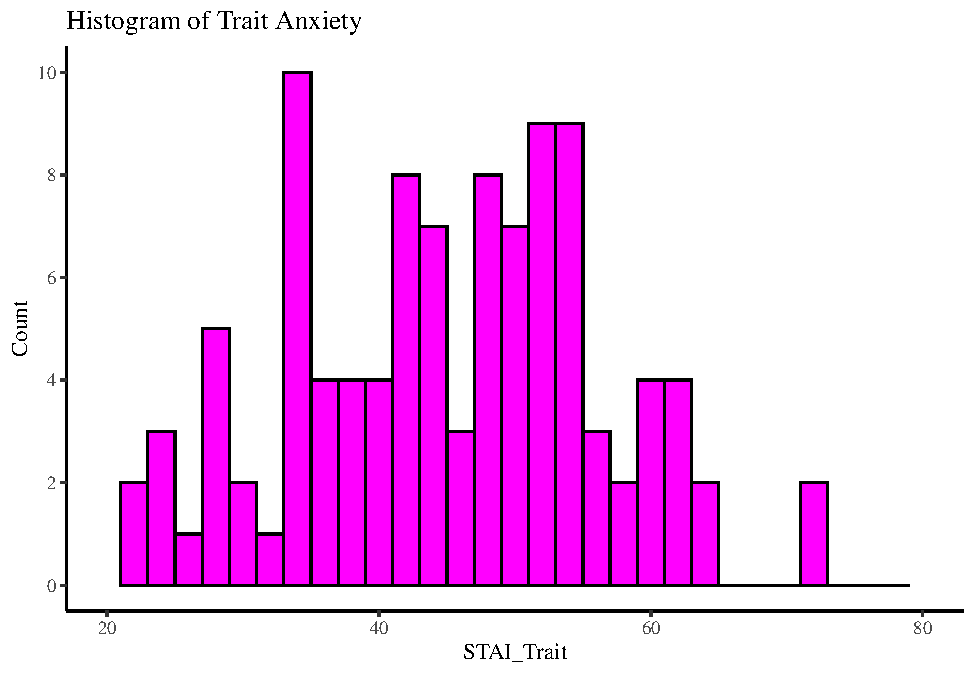
\includegraphics[width=1\linewidth]{d2m-Psychopathy_files/figure-latex/STAI-descriptives-1} \caption{Distribution of STAI-Trait scores in sample}\label{fig:STAI-descriptives-appendix}
\end{figure}

\begin{figure}[H]
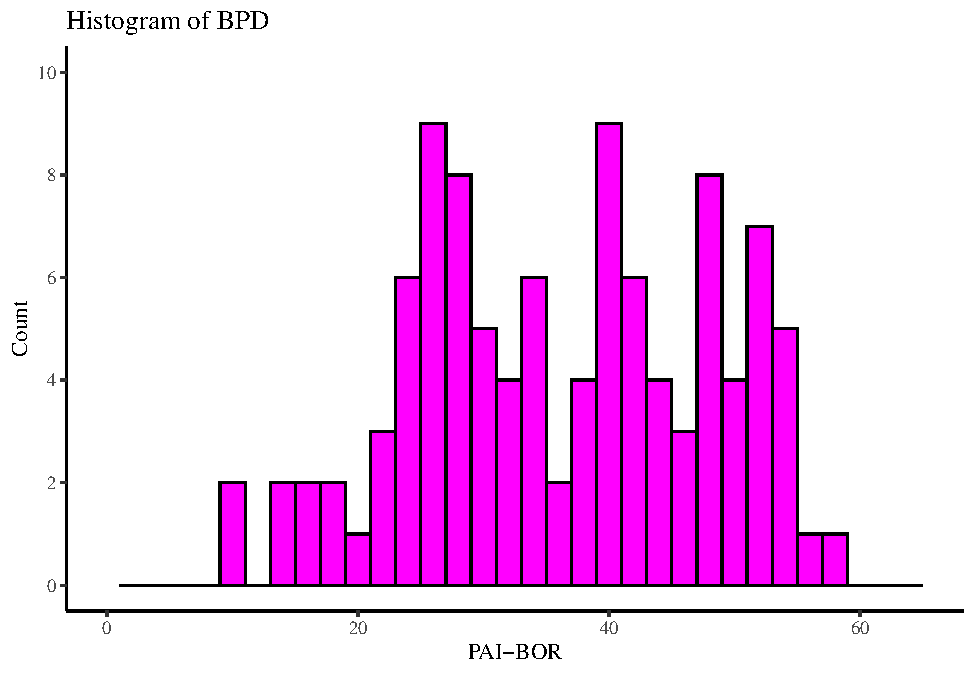
\includegraphics[width=1\linewidth]{d2m-Psychopathy_files/figure-latex/PAI-descriptives-1} \caption{Distribution of PAI-BOR scores in sample}\label{fig:PAIBOR-descriptives-appendix}
\end{figure}

\begin{figure}[H]
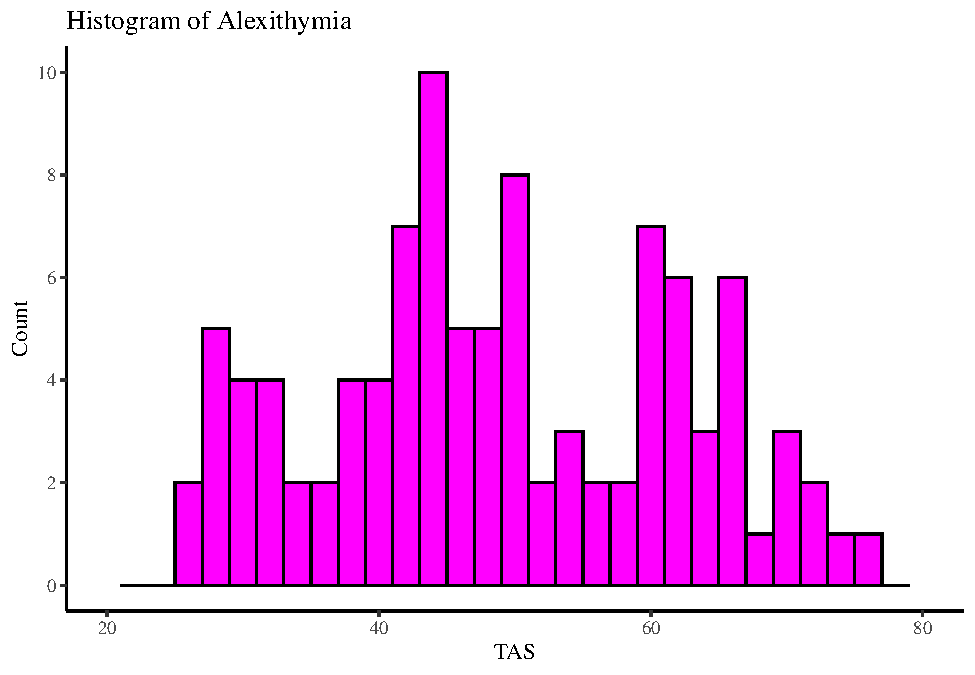
\includegraphics[width=1\linewidth]{d2m-Psychopathy_files/figure-latex/TAS-descriptives-1} \caption{Distribution of TAS scores in sample}\label{fig:TAS-descriptives-appendix}
\end{figure}

\begin{table}[!htbp] \centering 
  \caption{Preliminary Regression Results} 
  \label{tab:prelim-regression-output} 
\begin{tabular}{@{\extracolsep{1pt}}lccc} 
\\[-1.8ex]\hline 
\hline \\[-1.8ex] 
 & \multicolumn{3}{c}{\textit{Dependent variable:}} \\ 
\cline{2-4} 
\\[-1.8ex] & P-O Path & P-M Path & M-O Path \\ 
\\[-1.8ex] & (1) & (2) & (3)\\ 
\hline \\[-1.8ex] 
 PsychopathyXAnxiety & 0.373$^{***}$ & 0.660$^{***}$ &  \\ 
  & (0.092) & (0.074) &  \\ 
  & & & \\ 
 BPD &  &  & 0.471$^{***}$ \\ 
  &  &  & (0.087) \\ 
  & & & \\ 
 Constant & $-$0.000 & $-$0.000 & $-$0.000 \\ 
  & (0.091) & (0.074) & (0.087) \\ 
  & & & \\ 
\hline \\[-1.8ex] 
Observations & 104 & 104 & 104 \\ 
R$^{2}$ & 0.139 & 0.436 & 0.222 \\ 
Adjusted R$^{2}$ & 0.131 & 0.431 & 0.214 \\ 
Residual Std. Error (df = 102) & 0.932 & 0.755 & 0.887 \\ 
F Statistic (df = 1; 102) & 16.501$^{***}$ & 78.905$^{***}$ & 29.024$^{***}$ \\ 
\hline 
\hline \\[-1.8ex] 
\textit{Note:}  & \multicolumn{3}{r}{$^{*}$p$<$0.1; $^{**}$p$<$0.05; $^{***}$p$<$0.01} \\ 
\end{tabular} 
\end{table}


\end{document}
